\documentclass[twoside]{article}
\usepackage{amssymb}
\usepackage{amsthm}
\usepackage{amsmath}
\usepackage{amsfonts}
\usepackage[utf8]{inputenc}
\usepackage[spanish]{babel}
\usepackage{tikz}
\usepackage{centernot}
\usepackage{hyperref}
\usepackage{fancyhdr}
\usepackage{lipsum}
\usepackage{subcaption}
\hypersetup{
    colorlinks,
    citecolor=black,
    filecolor=black,
    linkcolor=black,
    urlcolor=black
}
\usepackage{xurl}
\usepackage[top=1in, bottom=1.5in, left=1in, right=1in]{geometry}
\pagestyle{fancy}
\fancyhead{}
\fancyhead[L]{\leftmark}
\fancyfoot{}
\fancyfoot[C]{\thepage}
\newcommand{\enquote}[1]{``#1''}
\usepackage{float}
\usepackage[parfill]{parskip}
\newcommand{\image}[2]{
\begin{figure}[H]
    \includegraphics[width=#1 cm]{../images/#2.png}
    \centering
\end{figure}
}

\title{Práctica 3 SWAP}
\author{XuSheng Zheng}
\date{}

\begin{document}

\maketitle
\tableofcontents
\newpage

\section{Creación de la tercera máquina}
Para esta práctica, necesitamos crear una tercera máquina virtual que nos servirá de balanceador. Para ello, especificamos los siguientes datos siguiendo los mismos pasos que en la práctica 1:
\image{8}{1}
Una vez instalada la máquina, necesitamos configurar la conexión a red. Lo hacemos de la misma manera que en la práctica 1:
\image{8}{2}
Y comprobamos con \textbf{ifconfig}:
\image{8}{3}


\section{Nginx}
Instalamos \textbf{nginx} en m3 mediante \textbf{apt-get} con los comandos del guion y comprobamos que está activado:
\image{8}{4}
Ahora procedemos a la configuración: en primer lugar deshabilitamos la funcionalidad de servidor web editando en \textit{/etc/nginx/nginx.conf} comentando la línea \textit{include /etc/nginx/sites-enabled/*;} :
\image{8}{5}
Creamos el archivo de configuración \textit{/etc/nginx/conf.d/default.conf} con los siguientes datos:
\image{8}{6}
Una vez guardado, reiniciamos el servicio \textbf{nginx}. Para comprobar el funcionamiento del balanceador, se ha modificado el archivo \textit{/var/www/html/swap.html} para que se pueda distinguir las máquinas:
\begin{figure}[H]
    \centering
    \begin{subfigure}{.5\textwidth}
        \centering
        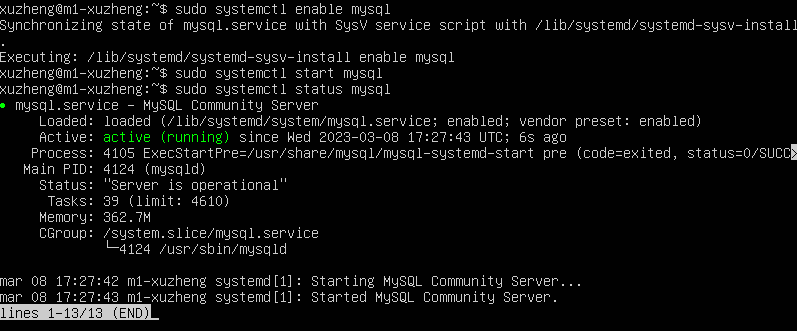
\includegraphics[width=7cm]{../images/10.png}
    \end{subfigure}%
    \begin{subfigure}{.5\textwidth}
        \centering
        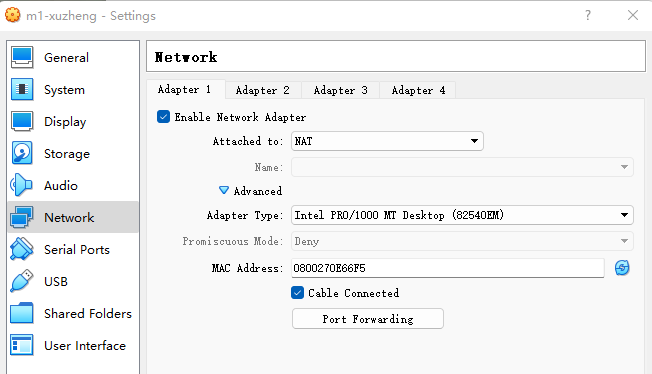
\includegraphics[width=7cm]{../images/11.png}
    \end{subfigure}
\end{figure}
Ahora podemos comprobar el funcionamiento de \textbf{nginx} usando \textbf{cURL} desde el anfitrión:
\image{8}{7}
En este caso hemos tratado las dos máquinas por iguales. Podemos dar más peso a la primera máquina mediante el modificador \textbf{weight}:
\image{8}{8}
Ahora de cada 3 peticiones, 2 serán atendidas por m1 y 1 por m2:
\image{8}{9}

\subsection{Opciones avanzadas}
Para evitar el conflicto de estados y sesiones entre los servidores, \textbf{nginx} permite dirigir las peticiones provenientes de un determinado IP al mismo servidor final mediante la opción \textbf{ip\_hash}. 

La directiva \textbf{keepalive} determina el número máximo de conexiones a servidores finales que se mantiene en caché y \textbf{keepalive\_requests} determina el número máximo de peticiones que pueden servir a través de estas conexiones, una vez que el número de peticiones exceda el máximo, la conexión se cerrará.
\image{8}{12}
Comprobamos el funcionamiento a través del anfitrión:
\image{8}{13}
Podemos que en este caso sólo sirve m2 pues estamos enviando a través del mismo IP.

Para gestionar caídas de los servidores podemos usar los comandos \textbf{max\_fails} para especificar el número máximo de intentos de comunicación fallidos antes de considerar al servidor no operativo y \textbf{fail\_timeout} para especificar el periodo de tiempo con el que se considera esos intentos. En el siguiente ejemplo consideramos que el servidor no será operativo si existen 3 intentos fallidos en un periodo de 30 segundos:
\image{8}{14}


\section{Haproxy}
Para este apartado, paramos y desactivamos \textbf{nginx} para evitar conflictos e instalamos \textbf{haproxy} mediante \textbf{apt-get}.
\image{8}{15}
Comprobamos que está activo:
\image{8}{16}
Pasamos ahora a configurar \textbf{haproxy}: añadimos al archivo \textit{/etc/haproxy/haproxy.cfg} las siguientes líneas para tener una configuración round-robin básica:
\image{8}{17}
Reiniciamos el servicio y comprobamos desde el anfitrión:
\image{6}{18}
Para dar más peso a determinados servidores, podemos usar la opción \textbf{weight} con números entre 0 y 256 en las líneas de \textbf{server}. Para tener la analogía con el apartado de \textbf{nginx}, asignamos a m1 el doble de carga que m2:
\image{8}{19}
Y comprobamos:
\image{6}{20}
Vemos que efectivamente m1 atiende 2 de las 3 peticiones.
\subsection{Opciones avanzadas}
Al igual que \textbf{nginx}, \textbf{haproxy} también permite el balanceo por IP mediante la opción \textbf{hash-type consistent}.

Además, \textbf{haproxy} permite 3 tipos de comprobaciones sobre el estado de los servidores:
\begin{itemize}
    \item Activo: por defecto en este caso \textbf{haproxy} intentará establecer una conexión TCP con el servidor final cada 2 segundos. Tras 3 conexiones fallidas se considerará que el servidor está caído y no se le enviará peticiones hasta que consiga 2 conexiones exitosas.
    \item Pasivo: similar a la opción \textbf{keepalive\_requests} de \textbf{nginx}, establece un límite de errores consecutivos que puede haber antes de dar por caído al servidor.
    \item Agente: mediante un agente externo del servidor final, \textbf{haproxy} puede controlar el estado con el que se encuentra el servidor.
\end{itemize}
En el siguiente ejemplo establecemos un máximo de 10 errores:
\image{8}{21}
Con \textbf{observe layer7} indicamos que se consideren todas las respuestas HTTP del servidor y con \textbf{on-error mark-down} indicamos que el servidor esta caído cuando se alcance los 10 errores.
Para comprobar el funcionamiento del balanceo por IP, mandamos peticiones desde el anfitrión:
\image{6}{22}
Podemos apreciar que todas las peticiones son atendidas por m1 pues provienen del mismo IP.



\newpage
\section{Bibliografía}
\begin{itemize}
    \item \url{http://nginx.org/en/docs/http/ngx_http_upstream_module.html}
    \item \url{http://www.haproxy.org/download/1.4/doc/configuration.txt}
    \item \url{https://serverfault.com/questions/113637/haproxy-roundrobin-weights}
    \item \url{https://www.haproxy.com/blog/client-ip-persistence-or-source-ip-hash-load-balancing}
    \item \url{https://www.haproxy.com/blog/how-to-enable-health-checks-in-haproxy}
    

    \item \url{https://serverfault.com/questions/123629/run-task-every-90-minutes-with-cron}
\end{itemize}

\end{document}
